\documentclass{acm_proc_article-sp}
\usepackage[latin1]{inputenc}
\usepackage[T1]{fontenc}
\usepackage{times}

\sloppy

\begin{document}

\title{On Component-Based Communication Systems\\for Clusters of
  Workstations}

\numberofauthors{2}

\author{
\alignauthor Ant�nio Augusto Fr�hlich\\
  \affaddr{Federal University of Santa Catarina}\\
  \affaddr{P.O. Box 476}\\
  \affaddr{88040-900 Florian�polis - SC, Brazil}\\
  \email{guto@inf.ufsc.br}
\alignauthor Wolfgang Schr�der-Preikschat\\
  \affaddr{University of Magdeburg}\\
  \affaddr{Universit�tsplatz 2}\\
  \affaddr{39106 Magdeburg, Germany}\\
  \email{wosch@ivs.cs.uni-magdeburg.de}
}

\maketitle
\thispagestyle{empty}

\begin{abstract}
  Most of the communication systems used to support high-performance
  computing in clusters of workstations have been designed focusing on
  ``the best'' solution for a certain network architecture. However, a
  definitive best solution, independently of how well tuned to the
  underlying hardware it is, cannot exist, for parallel applications
  communicate in quite different ways.  In this paper, we describe a
  novel design method that supports the construction of run-time systems
  as an assemblage of components that can be configured to closely match
  the demands of any given application. We also describe how this method
  has been deployed in the development of a communication system in the
  realm of \textsc{Epos}, a project that aims at delivering
  automatically generated application-oriented run-time support systems.
  The communication system in question has been implemented for a
  cluster of PCs interconnected with Myrinet, and corroborates the
  effectiveness of the proposed design method.
\end{abstract}

\category{D.4.4}{Operating Systems}{Communications Management}
\category{D.4.7}{Operating Systems}{Organization and
  Design}[application-oriented system design]
\category{D.2.13}{Software Engineering}{Reusable Software}[domain
  engineering]

\terms{Design, Experimentation, Performance}

\keywords{Cluster computing, High-performance computing,
  Applica\-tion-oriented operating systems}

\section{Introduction}

The parallel computing community has been using clusters of commodity
workstations as an alternative to expensive parallel machines for
several years by now. The results obtained meanwhile, both positive and
negative, often lead to the same point: inter-node communication.
Consequently, much effort has been dedicated to improve communication
performance in these clusters: from the hardware point of view,
high-speed networks and fast buses provide for low-latency and
high-bandwidth; while from the software point of view, \emph{user-level
  communication}~\cite{Bhoedjang:1998} enables applications to access
the network without operating system intervention, significantly
reducing the software overhead on communication. Combined, these
advances enabled applications to break the giga-bit-per-second bandwidth
barrier.

Nevertheless, good communication performance is hard to obtain when
dealing with anything but the test applications supplied by the
developers of the communication package. Real applications, not seldom,
present disappointing performance figures~\cite{npb}. We believe the
origin of this shortcoming to be in the attempt of delivering generic
communication solutions.  Most high-performance communication systems
are engaged in a ``the best'' solution for a certain architecture.
However, a definitive best solution, independently of how well tuned to
the underlying architecture it is, cannot exist, since parallel
applications communicate in quite different ways. Aware of this, many
communication packages claim to be ``minimal basis'', upon which
application-oriented abstractions can (have to) be implemented. Once
more, there cannot be a best minimal basis for all possible
communication strategies. This contradiction between generic and optimal
is consequently discussed in~\cite{Preikschat:1994}.

If applications communicate in distinct ways, we have to deliver each
one a tailored communication system that satisfies its requirements (and
nothing but its requirements). Of course we cannot implement a new
communication system for each application, what we can do is to design
the communication system in such a way that it becomes possible to
tailor it to any given application. In the \emph{Embedded Parallel
  Operating System} (\textsc{Epos}) project~\cite{Froehlich:ehpc:1999},
we developed a novel design method that is able to accomplish this duty.
\textsc{Epos} consists of a collection of components, a component
framework, and tools to support the automatic construction of a variety
of run-time systems, including complete operating systems.

The particular focus of this paper is on \textsc{Epos} communication
system, which has been implemented for a cluster of PCs interconnect by
a Myrinet high-speed network. In the next sections, the
\emph{Application-Oriented System Design} method will be introduced,
followed by a case study of its applicability to design a communication
system.  The implementation of this communication system will be
discussed later, including a preliminary performance evaluation. The
paper is closed with authors' conclusions.


\section{Application-Oriented System\\Design}

\emph{Application-Oriented System Design} (AOSD) is a novel operating
system\footnote{The term ``operating system'' is used here in its
  broadest meaning, encompassing all kinds of run-time support systems.}
design method that, as the name suggests, is strongly compromised with
applications. Its main goal is to produce run-time support systems that
can be tailored to fulfill the requirements of particular applications.
Accomplishing this task begins with the decomposition of the target
domain in abstractions that are natural to application programmers. This
is exactly the decomposition strategy promoted by \emph{Object-Oriented
  Design}~\cite{Booch:1994} and may sound obvious to application
designers, but most system designers simply neglect the problem domain
and let implementation details, such as target architecture, programming
languages, and standardized interfaces, guide the design
process~\cite{Pike:2000}. Application programmers, not seldom, get
run-time systems that barely resemble the corresponding domain.

The next step is to model software components that properly represent
the abstractions from the decomposed domain. Extensive components, that
encapsulate all perspectives of an abstraction in a single entity, are
not an alternative, since we want components to closely match the
requirements of particular applications. A more adequate approach would
be to apply the commonality and variability analysis of
\emph{Family-Based Design}~\cite{Parnas:1976} to yield a family of
abstractions, with each member capturing a significant variation and
shaping a component.  Nevertheless, this approach has the inconvenient
of generating a large number of components, thus increasing the
complexity of the composition process.  We handle this drawback by
exporting all members of a family through a single \emph{inflated
  interface}.  In a system designed accordingly, adequate members of
each required family could be automatically select by a tool that
performs syntactical analysis of the corresponding application's source
code.

Another important factor to be considered while modeling abstractions is
scenario independence. When a designer realizes, for instance, that a
communication mechanism may have to be specialized in order to join a
multithreaded scenario, he has to choose between modeling a new family
member and capturing this scenario dependency in a separate construct.
Allowing abstractions to incorporate scenario dependencies reduces their
degree of reusability and produces an explosion of scenario-dependent
components. Therefore, an application-oriented design should try to
avoid it, only allowing those variations that are inherent to the family
to shape new members. The resulting \emph{scenario-independent
  abstractions} shall be reusable in a larger variety of scenarios, some
of them unknown at the time they were modeled.

Scenario specificities, in turn, can be captured in constructs like the
\emph{scenario adapters} described in~\cite{Froehlich:sci:2000}. Because
scenario adapters share the semantics of collaborations in
\emph{Collabo\-ra\-tion-Based Design}~\cite{Reenskaug:1992}, one could say
that an abstraction collaborates in a scenario. This separation of
abstractions and scenario aspects is also pursued by
\emph{Aspect-Oriented Programming}~\cite{Kiczales:1997}, nevertheless,
though it provides means to support this separation, it does not yet
feature a clear domain decomposition strategy.

\begin{figure}
\centering
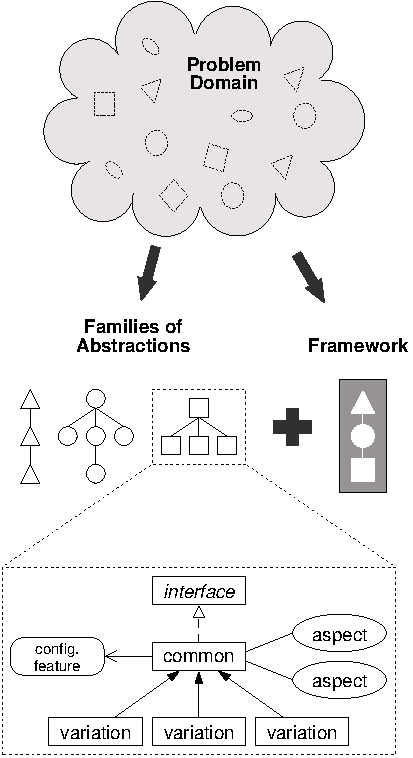
\epsfig{file=pdf/aosd.pdf, scale=0.8}
\caption{An overview of Application-Oriented System Design.
  \label{fig:aosd}}
\end{figure}

The primary strategy of Application-Oriented System Design to add
functionality to a family of abstractions is the definition of new
family members, but sometimes it is desirable to extend the behavior of
all members of a family at once. For example, a family of network
abstractions might feature multicasting and error detection at
application's convenience. Instead of specializing each family member,
what would double the cardinality of the family, such extensions could
be factorized as \emph{configurable features}.  Like scenario aspects,
configurable features modify the behavior of all members of a family
when activated, but, unlike those, are not transparent.  One could say
that scenario aspects have ``push'' semantics, while configurable
features have ``pull''. A configurable feature encapsulates common data
structures and algorithms that are useful to implement a feature in the
context of a family, but leave the actual implementation up to each
family member.  Abstractions are free to reuse, extend, or override what
is provided in a configurable feature, but are requested to behave
accordingly when the feature is enabled.

After decomposing the problem domain in scenario-indepen\-dent
abstractions and scenario-adapters, organizing the solution domain
accordingly becomes straightforward. \emph{Inflated interfaces} hide
most details of the solution domain by exporting all members of a family
of abstractions, as well as the corresponding scenario adapters, through
a single interface. Since these interfaces emanate directly from the
problem domain, application programmers should feel comfortable to use
them. What is missing to deliver a true application-oriented run-time
system is a way to assemble components together correctly and
efficiently. By correct assembly we mean preserving the individual
semantics of each component in the presence of others and under the
constraints of an execution scenario.  By efficient assembly we mean
preserving their individual efficiency in the resulting composite.

One possibility to produce the desired compositions is to capture a
reusable system architecture in a \emph{component framework}. A
framework enables system designers to predefine the relationships
between abstractions and therefore can prevent misbehaved compositions.
Furthermore, a framework defined in terms of scenario adapters
(figure~\ref{fig:framework}) can achieve a high degree of adaptability.
Efficient composition can be accomplished if the framework uses
\emph{Generative Programming} techniques~\cite{Czarnecki:2000}, such as
\emph{static metaprogramming}.  Since static metaprograms are executed
at compile-time, a statically metaprogrammed framework can avoid most of
the overhead typical of traditional object-oriented frameworks.  It is
also important to notice that, though component composition would take
place at compile-time, nothing would prevent components from using
dynamic reconfiguration mechanisms to internally adapt themselves.

\begin{figure}[h]
\centering
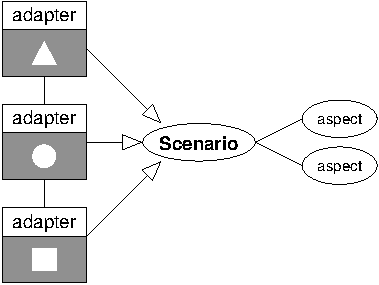
\epsfig{file=pdf/framework.pdf, scale=0.8}
\caption{A component framework based on scenario adapters.
  \label{fig:framework}}
\end{figure}

In brief, \emph{Application-Oriented System Design} is a multiparadigm
design method that supports the construction of customizable run-time
support systems by decomposing the system domain in families of
reusable, scenario-independent abstractions and the corresponding
scenario adapters. Reusable system architectures are modeled as
component frameworks that can guide the compilation of the target
system. Application programmers interact with the system through
inflated interfaces, without having to know details about the
organization of families or scenarios.


\section{The Design of an Application-Oriented Communication System}

We applied Application-Oriented System Design to develop a communication
system for clusters of workstations in the realm of project
\textsc{Epos}. By decomposing the domain of high-performance cluster
communication, we obtained the families of abstractions shown in
figure~\ref{fig:epos_comm}.  Application processes communicate with each
other using a \texttt{Communicator}, which acts as an interface to a
communication \texttt{Channel} implemented over a \texttt{Network}.  The
messages sent through a \texttt{Communicator} can be specified as
sequences of bytes of a known length, or they can be covered by an
\texttt{Envelope}.

\begin{figure}[h]
\centering
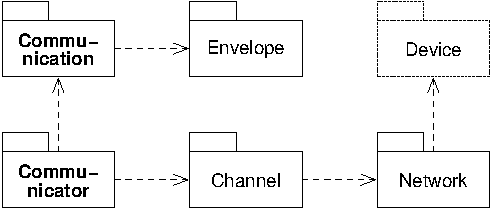
\epsfig{file=pdf/epos_comm.pdf, scale=0.8}
\caption{Families of abstractions concerning \textsc{Epos}
  communication system.\label{fig:epos_comm}}
\end{figure}

\subsection{Communicators}

A \emph{communicator} is an end-point for a communication channel that
enables application processes to exchange data with each other.
Therefore, when an application selects a communicator, it implicitly
designates the kind of communication channel that will be used.
Communicators, like most other \textsc{Epos} abstractions, are assigned
to tasks, thus being shared by their threads.  Communicators are
realized in \textsc{Epos} by the \texttt{Communicator} family of
abstractions shown in figure~\ref{fig:epos_comm_communicator}.

\begin{figure}
\centering
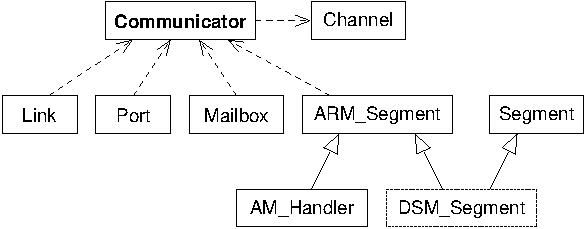
\epsfig{file=pdf/epos_comm_communicator.pdf, scale=0.8}
\caption{\textsc{Epos} family of communicators.
  \label{fig:epos_comm_communicator}}
\end{figure}

The \texttt{Link} member of the \texttt{Communicator} family realizes an
end-point for logical connections between processes that carry byte
streams. The \texttt{Port} and \texttt{Mailbox} members realize
end-points for a communication channel in which datagrams flow, but a
port always belongs to a single task, while mailboxes can be shared
among tasks.

The \texttt{ARM\_Segment} (\emph{Asynchronous Remote Memory Segment})
member of the \texttt{Communicator} family realizes an end-point for a
communication mechanism that supports asynchronous access to a memory
segment in a remote node.  This mechanism is asynchronous because
processes manipulating an \texttt{ARM\_Segment} are not implicitly
synchronized and can corrupt the data in that segment. Data read from a
remote segment becomes local and private to the reading process.  If
necessary, synchronization has to be achieved by other means (e.g.
distributed semaphores). In order to use this communicator, a process
specifies a memory segment on a remote node that has been previously
exported by its owner.  It can then invoke operations to read from and
to write to this segment (asynchronous remote memory segments are not
mapped into the address space of processes).

The \texttt{AM\_Handler} (\emph{Active Message Handler}) member of the
\texttt{Communicator} family realizes an end-point for active
messages~\cite{Eicken:1992}. The basic idea behind this concept is that
a message, besides transporting data, also carries a reference to a
handler that is invoked, in the context of the receiving process, to
handle the message upon arrival. This kind of communication is sometimes
called single-sided because the receive operation is not explicitly
expressible. For this mechanism to work properly, means must be provided
to the sending process so it can specify a handler that is valid in the
context of the destination process. The most typical answer to this
issue is to deploy active messages in an SPMD (\emph{Single Program,
  Multiple Data}) environment, in which all processes have an equivalent
address space.  However, indirection mechanisms and the exchange of
handler references using other communication mechanisms are also
possible.

Active messages have been modeled in \textsc{Epos} in such a way that
communication is hidden behind a remote handler invocation, with
messages being indirectly exchanged as arguments to the handler. When a
process instantiates an \texttt{AM\_Handler}, it supplies a reference to a
handler on a remote process.  Afterwards it can invoke the handler
supplying arguments that are transparently marshaled in a message and
delivered to the remote handler.

The \texttt{DSM\_Segment} member of the \texttt{Communicator} family,
which realizes a \emph{Distributed Shared Memory}~(DSM) mechanism for
\textsc{Epos}, has been modeled as an extension of the
\texttt{ARM\_Segment} communicator and of a member of the
\texttt{Segment} family of memory segments.  Unlike
\texttt{ARM\_Segments}, however, \texttt{DSM\_Segments} can be attached
to the address space of processes, dispensing with explicit read and
write operations. It also comprises mechanisms to grant data coherence.
This communicator enables application programmers to write parallel
applications for distributed memory machines as if they were shared
memory ones.


\subsection{Channels}

A communication \emph{channel} is the entity effectively responsible for
inter-process communication in \textsc{Epos}. It uses network resources
to build a logical communication channel through which messages can be
exchanged.  A channel implements a communication protocol that,
according with the \emph{Basic Reference Model for Open Systems
  Interconnection}~(ISO/OSI-RM)~\cite{osi}, would be classified at level
four (transport). \textsc{Epos} family of communication channels is
depicted in figure~\ref{fig:epos_comm_channel}.  It was modeled as a
dissociated family, whose members are indirectly accessed through the
corresponding members of the \texttt{Communicator} family.
  
\begin{figure}
\centering
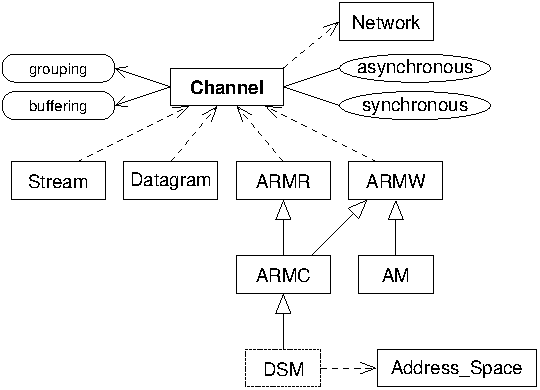
\epsfig{file=pdf/epos_comm_channel.pdf, scale=0.8}
\caption{\textsc{Epos} family of communication channels.
  \label{fig:epos_comm_channel}}
\end{figure}

A communication channel has an implicit capacity.  Trying to insert a
message into a saturated channel causes the transmitter to wait until
the channel can accommodate the message.  Likewise, the attempt the
extract a message from an empty channel causes the receiver to wait
until a message is available.  Whether a thread waiting on a channel
performs busy or idle waiting hinges on the related configurable feature
from the \texttt{CPU\_Scheduler} family of abstractions.
Notwithstanding this, a channel can have its capacity extended by
enabling the \texttt{buffering} configurable feature. In this case,
messages sent through a saturate channel are accumulated for posterior
handling.

Sometimes it is desirable to fork a channel, so that a transmitted
message is simultaneously multicasted to several receivers, or
broadcasted to all receivers. The collective operations used in many
parallel applications could be considerably optimized in this way.
\textsc{Epos} allows a channel to be forked when the \texttt{grouping}
configurable feature is enabled. In this case, special identifiers are
supplied to designate a group of communicators as the recipient of a
message. The effect of \texttt{buffering} and \texttt{grouping} configurable
features on a channel is illustrated in figure~\ref{fig:channels}.

\begin{figure}[h]
\centering
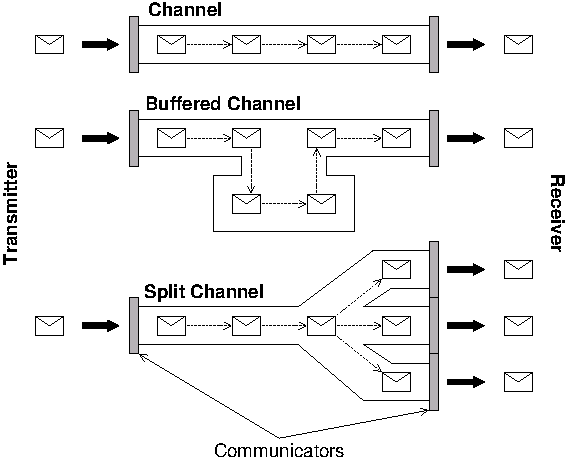
\epsfig{file=pdf/channels.pdf, scale=0.8}
\caption{The effect of configurable features \texttt{buffe\-ring}
  and \texttt{grouping} on communication channels.
  \label{fig:channels}}
\end{figure}

The \texttt{synchronous} scenario aspect yields an execution scenario in
which the operations used to inject a message into a channel only
conclude when the message is extracted from the channel at the
receiver's side. In a synchronous communication scenario, processes
involved in a message exchange are said to make a ``rendezvous''.
Conversely, the \texttt{asynchronous} scenario aspect modifies these
operations so they conclude as soon as the delivery of a message is
negotiated. If the \texttt{buffering} configurable feature is enabled, this
is achieved by copying the message into a buffer and scheduling it for
delivery.  Otherwise, the sender is supposed not to modify the message
until indicated to do so. An operation is provided that enables a
process to check for this condition.

The \texttt{Stream} member of the \texttt{Channel} family realizes a
connection-oriented channel that can be used to transfer streams of
bytes. It pairs up with the \texttt{Link} communicator. The
\texttt{Datagram} member realizes a channel that supports the
transmission of \emph{datagrams}. It has two possible end-points:
\texttt{Port} and \texttt{Mailbox}. Three members concern asynchronous
access to a remote memory segment: \texttt{ARMR}, \texttt{ARMW}, and
\texttt{ARMC}. They realize communication channels respectively for
reading, writing, and copying (reading and writing) from/to a remote
memory segment and are delivered to applications through the
\texttt{ARM\_Segment} communicator.  The reason to model these three
members separately is that read and write operations can be optimized if
they do not occur simultaneously.

The \texttt{AM} (\emph{Active Message}) channel specializes \texttt{ARMW} to
introduce the concept of a message handler that is automatically invoked
when the message reaches its destination. It pairs up with the
\texttt{AM\_Handler} communicator. The communication channel used to
support distributed shared memory would specialize the \texttt{ARMC}
channel in order to map it to the address space of processes. 


\subsection{Networks}

A communication channel is, at last, an abstraction of a network, in
that networks provide the physical means to build logical channels. The
idiosyncrasies of each network technology, however, could require the
members of the \texttt{Channel} family to be specialized too often. This
picture was prevented in \textsc{Epos} by modeling networks as members of a
uniform family of abstractions, so that all networks are equivalent from
the standpoint of channels.

The uniform design of the \texttt{Network} family, which is outlined in
figure~\ref{fig:epos_comm_network}, shall not subdue special features
delivered by a particular network, since abstractions in this family
implement high-level transport services that are seldom implemented by
the hardware.  The virtual networks in this family can use special
services provided by the network to optimize the implementation of such
transport services.  Some of these special features are used to
implement the configurable features modeled for the family.

\begin{figure}[b]
\centering
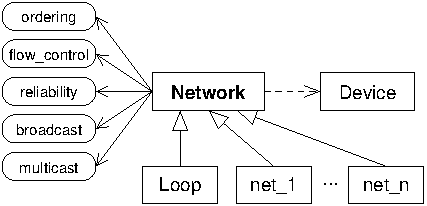
\epsfig{file=pdf/epos_comm_network.pdf, scale=0.8}
\caption{\textsc{Epos} family of networks.
  \label{fig:epos_comm_network}}
\end{figure}

The \texttt{Network} family features a member for each network
technology supported in the system (e.g. Ethernet and Myrinet). Each
member encapsulates a physical network \texttt{Device}. The family also
features a \texttt{Loop} device that is used to establish a
communication channel between processes executing on the same node.  In
principle, abstractions in this family are used indirectly through a
communicator, but they are also made available for the convenience of
applications that need, for instance, to implement special communication
protocols.

A set of configurable features, corresponding to operational modes, was
modeled for the \texttt{Network} family. These features are interpreted as
follows: \texttt{ordering} requires messages sent through a network to be
delivered at the destination in the same order they were sent;
\texttt{flow\_control} requires a network abstraction to implement flow
control; \texttt{reliability} requires a network to assure error-free
delivery of messages; \texttt{broadcast} enables the interpretation of
broadcast addresses, so messages can be broadcasted to all hosts in the
local network; \texttt{multicast} enables the interpretation of multicast
addresses, causing a message to be delivered at multiple hosts. These
configurable features are usually specialized for each family member to
profit from eventual hardware support.


\subsection{Message Envelopes}

The members of the \texttt{Communicator} family can be used to exchange
unstructured messages in the form of sequences of bytes of a certain
length. However, it might be adequate for some applications to count on
an \emph{envelope} abstraction to cover a message before sending it.
Such an envelope would be allocated from the operating system, loaded
with one or more messages, and then inserted into a communication
channel through a communicator.  An envelope allocated by the operating
system would enable several optimizations, ranging from cache alignment
to zero-copy processing. Besides, additional information can be put in
the envelope to describe and protect messages. After all, an envelope
would enable a comfortable syntax to express communication in
object-oriented applications, for example:

\begin{verbatim}
  Envelope envelope(recipient, length);
  envelope << "Hello world!";
  communicator << envelope;
\end{verbatim}

\textsc{Epos} supports the concept of \emph{message envelope} through the
\texttt{Envelope} uniform family of abstractions represented in
figure~\ref{fig:epos_comm_envelope}.  The maximum length of message that
an envelope can hold is specified when it is instantiated, while the
effective length of the message(s) it contains is dynamically
determined.  An envelope must be addressed before it is posted. 

\begin{figure}[b]
\centering
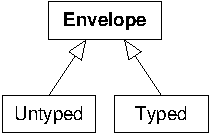
\epsfig{file=pdf/epos_comm_envelope.pdf, scale=0.8}
\caption{\textsc{Epos} family of message envelopes.
  \label{fig:epos_comm_envelope}}
\end{figure}

The \texttt{Envelope} family comprises two members: \texttt{Untyped} and
\texttt{Typed}.  The former realizes a simple message envelope that can
be used to gather messages before sending, while the latter collects
type information for each message inserted to enable format conversions
on heterogeneous systems. A \emph{secure envelope} was not modeled due
to the characteristics of a dedicated computing system, which usually do
not require encryption nor authentication of messages.


\subsection{Scenario Aspects}

Application-Oriented System Design is particularly concerned with
scenario independence. When a domain entity is identified,
considerations about its origin are made in order to decide whether it
will shape an abstraction or a scenario aspect. \textsc{Epos} scenario
aspects were modeled in accordance with this principle, yielding
reusable pieces of software that can be controllably applied to the
system abstractions described in the previous section.
Figure~\ref{fig:epos_asp} shows scenario aspects that apply to
\textsc{Epos} communication system.

\begin{figure}[h]
\centering
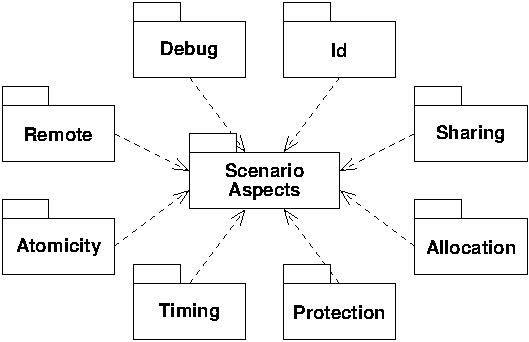
\epsfig{file=pdf/epos_asp.pdf, scale=0.8}
\caption{Families of scenario aspects concerning \textsc{Epos}
  communication system.\label{fig:epos_asp}}
\end{figure}

\begin{description}
  
\item[Identification:] instances of \textsc{Epos} abstractions can be
  identified in four ways: (a) by its address in memory in single-task
  scenarios; (b) by a pair \texttt{(type, unit)} in stand-alone
  multitasking scenarios; (c) by a tuple \texttt{(host, type, unit)} in
  distributed scenarios; and (d) by a sparse capability of the type
  \texttt{(host, type, unit, rand)} for protected distributed scenarios.
  Although embedding location in identifiers complicates the migration
  of objects in a distributed environment, \textsc{Epos} opted for this
  solution because it is efficient and fulfills the demands of most
  parallel systems.
  
\item[Sharing:] \textsc{Epos} abstractions can be shared both in local
  and distributed environments. The family of sharing scenario aspects
  features two members: the first performs reference counting, while the
  second extends the family to support possession lists.  When one of
  these aspects is enabled, system abstractions gain two extra
  constructors that are used to designate sharing.  The first is the
  ordinary copy constructor, which takes a reference to an existing
  system object as argument and returns a share to that object.  This
  constructor is restricted to share abstractions inside a single
  address space. The second constructor takes an identifier as argument
  and therefore can be used independently of locality, inclusive to
  share remote objects.  A C++ program could deploy these constructors
  as follows:

\begin{verbatim}
  Abstraction instance;
  Abstraction share1(instance);
  Abstraction share2(share1.id());
\end{verbatim}
  
\item[Allocation:] in order to reduce run-time overhead, \textsc{Epos}
  abstractions can be allocated in advance during system initialization,
  so that applications get all resources they will need by the time they
  start execution.  This is accomplished by a scenario aspect that
  interacts with \textsc{Epos} initialization programs to pre-allocate
  vectors of objects that are controlled by special allocators.
  Otherwise, a counterpart scenario aspect takes care for dynamic
  allocation.
  
\item[Protection:] \textsc{Epos} supports a protected execution scenario
  for applications. This scenario profits from the capability
  identification aspect to build an access control mechanism similar to
  the one described in~\cite{Mullender:1986}.
  
\item[Timing:] two scenario aspects concerning timing have been modeled
  for \textsc{Epos} communication system. One supports the specification
  of time-outs for abstractions' operations; the other inserts delays on
  operations to balance execution time in heterogeneous systems.
  
\item[Atomicity:] when multiple threads are allowed to execute in
  parallel, it its possible that they simultaneously ``enter'' the
  operating system, i.e.  pass to execute operating system code to
  accomplish a system service.  \textsc{Epos} handles the
  synchronization pitfalls brought about by reentrance ensuring that
  system operations are \emph{atomic}.  In this way, transformations of
  the state of system objects either occur completely or do not occur at
  all.
  
\item[Remote Invocation:] in a distributed environment, processes may
  need to access system resources residing on remote nodes. In order to
  do so, an application would have to create a process on each node
  containing useful resources and deploy a \texttt{Communicator} to
  interact with them.  However, \textsc{Epos} eliminates the burden of
  explicit message passing for accessing remote resources with a
  \emph{Remote Object Invocation}~(ROI) mechanism similar to the one
  described in~\cite{Levy:1991}.  Such a mechanism hides inter-process
  communication behind ordinary method invocations, so that processes
  can transparently access remote resources.  This scenario aspect that
  can be transparently applied to virtually any abstraction.
  
\item[Debugging:] being able to trace the invocation of system
  operations, or to watch the state of system abstractions, can be
  useful to debug application programs.  Likewise, being able to
  summarize how much time an application spends with each system
  abstraction may be a source of optimization. \textsc{Epos} supports
  these features through a family of scenario aspects.

\end{description}


\subsection{System Generation}

When completely implemented for a variety of network architectures,
\textsc{Epos} communication system will yield a large number of
components that will be stored in a repository together with several
other subsystems. With such a large number of components, selecting and
configuring the right ones in order to produce an application-oriented
system may become a defying activity, even when assisted by visual
tools. Hence, Application-Oriented System Design proposes all members of
a family to be exported through a single, inflated interface.  In this
way, application programmers can design and implement their applications
referring to fewer interfaces and ignoring the particular properties of
each component.  Actually, the programmer catches a comprehensive
perspective of the family, as though a super-component was available,
and uses the operations that better fulfill his requirements\footnote{In
  case an application programmer with enough expertise about the system
  wishes to extend a component, or bypass automatic configuration, the
  individual interfaces of each family member are also made available.}.
As an example, the inflated interface of the \texttt{Communicator}
family is depicted in figure~\ref{fig:communicator_int}.

\begin{figure}
  \centering
  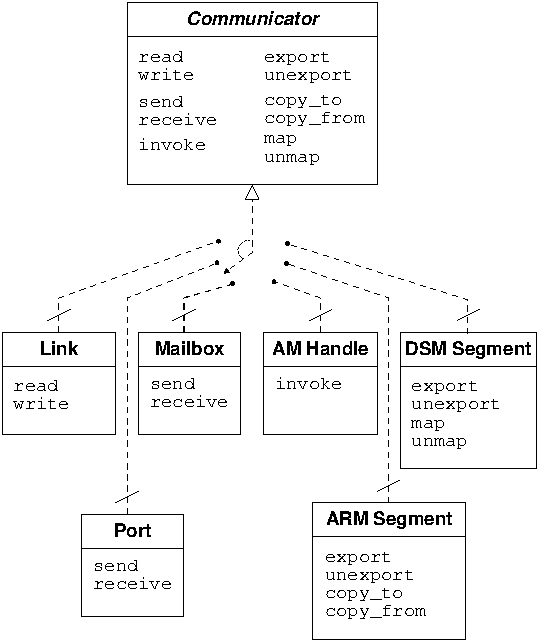
\epsfig{file=pdf/communicator_int.pdf, scale=0.8}
  \caption{The Communicator inflated interface and its realizations.
    \label{fig:communicator_int}}
\end{figure}

The process of binding an inflated interface to one of its realizations
can be automated if we are able to clearly distinguish one realization
from another.  In \textsc{Epos}, we identify realizations through the
signatures of their methods, so that syntactical analysis of application
source code can identify which of the realizations are needed. If two
realizations present the same set of signatures, as with \texttt{Port}
and \texttt{Mailbox} in figure~\ref{fig:communicator_int}, syntactical
analysis might not be enough to decide for one of them, and user
intervention may be required. Nevertheless, although \texttt{Port} and
\texttt{Mailbox} differ only semantically\footnote{Both \texttt{Port}
  and \texttt{Mailbox} support multiple senders, but the first supports
  a single receiver, while the second support multiple receivers too.},
the syntactical analysis of other components may render one possibility
invalid. For example, if the application is known to execute on a
single-task-per-node basis, a scenario with multiple receivers is not
possible, breaking the tie in favor of \texttt{Port}.

The set of selected family members, in addition to information obtained
from the user, defines the execution scenario for the application. As
proposed by Application-Oriented System Design, scenario peculiarities
are applied to abstractions by means of scenario adapters. In
\textsc{Epos}, a scenario adapter wraps an abstraction as to enclose
invocations of its operations between the \texttt{enter} and
\texttt{leave} scenario primitives (see
figure~\ref{fig:scenario_adapter}). Besides enforcing scenario specific
semantics, a scenario adapter can extend the state and behavior of an
abstraction, for it inherits from both scenario and abstraction. For
example, all abstractions in a scenario could be tagged with a
capability, without internal modifications, by associating the
capability with the corresponding scenario.

\begin{figure}
  \centering
  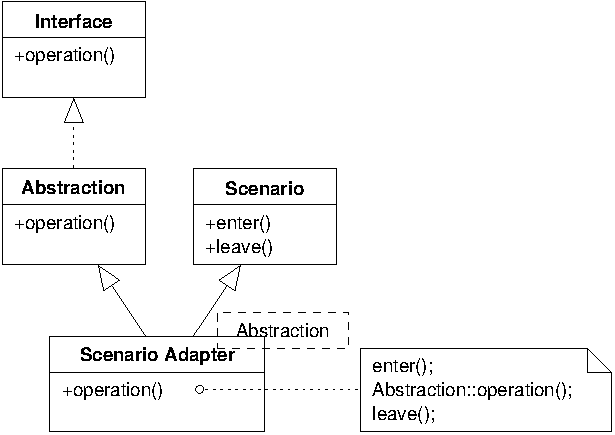
\epsfig{file=pdf/scenario_adapter.pdf, width=\columnwidth}
  \caption{The structure of a scenario adapter.
    \label{fig:scenario_adapter}}
\end{figure}

\textsc{Epos} statically metaprogrammed framework is defined around a
collection of interrelated scenario adapters. As shown in
figure~\ref{fig:scenario_adapter}, scenario adapters are designed as
parametrized classes that take a component (abstraction) as parameter.
Hence they can act as placeholder for components in the framework. In
order to generate a system, information about the mapping of inflated
interfaces to realizations, and also about system-wide properties such
as target architecture and protection, are passed as input to the
metaprogram.  The resulting system would include only the components
needed to support the corresponding application in the respective
execution scenario.


\section{The Implementation of the\\Communication System}
 
The design of \textsc{Epos} described above is being implemented as a
collection of components, a framework, and a set of tools that support
automatic generation of application-oriented run-time systems. Currently
the system can run in two modes: native on \textsc{ix86} computers, and
guest on \textsc{Linux} systems.  The \textsc{ix86}-native version can
be configured either to be embedded in the application (single-task), or
as $\mu$-kernel (multi-task), while the \textsc{Linux}-guest version
comprises a library and kernel loadable modules.

Components are being implemented in C++ and described in XML. The XML
description is used by the tools that support automatic system
generation. The framework is also implemented in C++, but mainly with
its built-in static metalanguage.  The tools to proceed syntactical
analysis of applications, to configure the target system, and to check
configuration dependencies are made available to users through a
compiler wrapper similar to \texttt{mpicc}. This enables users to
implicitly generate the run-time system during the compilation of
applications.  Nevertheless, if these tools fail to configure the
system, user intervention is requested via an interactive graphical tool
that supports configuration adjustments by feature
selection\footnote{The same tool can be used to tailor the system
  manually.}.

\textsc{Epos} family of communication abstractions is currently being
implemented for the Myrinet high-speed network~\cite{Boden:1995}. So
far, we concluded the implementation of the \texttt{Port} and
\texttt{Mailbox} \texttt{Communicators}, the \texttt{Datagram}
\texttt{Channel}, the \texttt{Myrinet} \texttt{Network}, and a mechanism
to support \emph{remote object invocation} (ROI). These components can
be adapted to the following scenarios: \texttt{Protected},
\texttt{Multitask}, \texttt{Multithread}, and \texttt{Global}. The
\texttt{Protected} scenario ensures that only authorized agents gain
access to abstractions. The \texttt{Multitask} and \texttt{Multithread}
scenarios adapt abstractions to execute in the presence of multiple
tasks and threads. The \texttt{Global} scenario adapts abstractions to
interact in a cluster-wide environment of active objects, hiding
communication behind ordinary method invocations.

With these components we generated a couple of appli\-cation-oriented
run-time systems. One of them supports two simple applications that
communicate intensively in a producer/consumer fashion. For this
purpose, they use the \texttt{Port Communicator}, the \texttt{Datagram
  Channel}, and the \texttt{Myrinet Network}.  Figures~\ref{fig:latency}
and~\ref{fig:bandwidth} show respectively the latency and the bandwidth
available to these applications in both \textsc{ix86}-native and
\textsc{Linux}-guest modes. The hardware test-bed for this measurements
consisted of two PCs connected to the same Myrinet switch. Each PC has a
266 MHz Pentium II processor, 128 MBytes of memory (10 ns DRAM) on a 66
MHz bus, and a 32-bits Myrinet NIC on a 33 MHz PCI bus.

\begin{figure}[t]
  \centering
  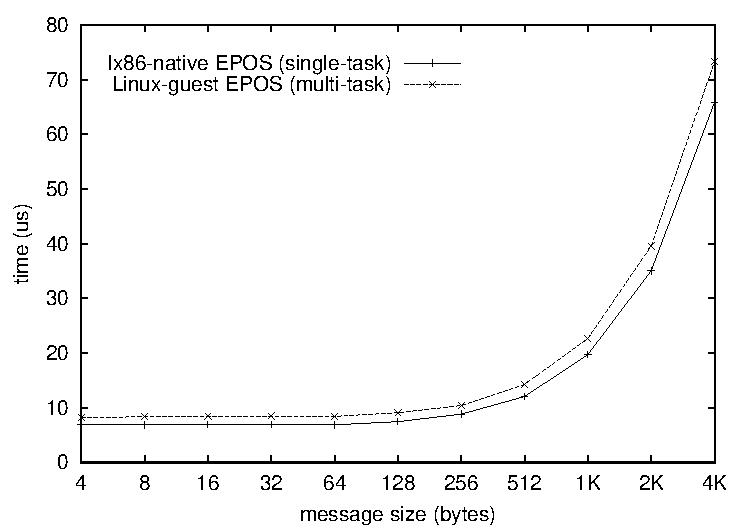
\epsfig{file=pdf/latency.pdf, width=\columnwidth}
  \caption{\texttt{Port/Datagram/Myrinet} one-way latency.
    \label{fig:latency}}
\end{figure}

\begin{figure}
  \centering 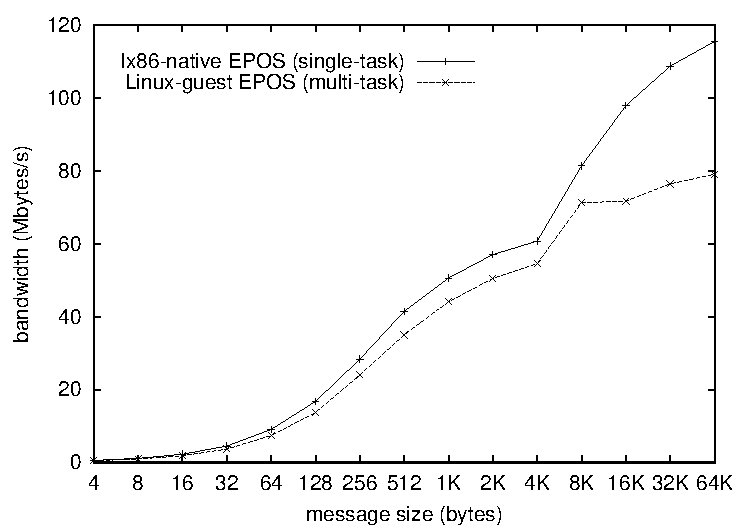
\epsfig{file=pdf/bandwidth.pdf, width=\columnwidth}
  \caption{\texttt{Port/Datagram/Myrinet} one-way bandwidth.
    \label{fig:bandwidth}}
\end{figure}

The difference in favor of the \textsc{ix86}-native version arises from
the contiguous memory allocation method adopted, which allows the DMA
engines on the Myrinet card to be programmed with logical addresses and
eliminates an additional message copy into a system DMA buffer. This
difference could have been even more expressive if the applications were
multithreaded, since the extra copy would have concurred with
application threads for processor time and especially for memory
bandwidth.  Nevertheless, most parallel applications execute on a
single-task-per-node basis and will benefit from the single-task
versions of \textsc{Epos}. Other communication systems, such as Active
Messages~\cite{Lumetta:1997}, Fast Messages~\cite{Pakin:1997},
PM~\cite{Tezuka:1997}, and BIP~\cite{Prylli:1998}, run exclusively on
top of ordinary operating systems, such as \textsc{Unix} or
\textsc{Windows NT}, and have no alternative to escape the extra copy
than making a system call to translate logical addresses into physical
ones, what is usually even more time consuming\footnote{Sharing system
  DMA buffers with applications is not really an alternative, because
  they are usually restricted in size and will not be able accommodate
  the large data structures typical of parallel applications. It would
  most likely result in the application performing the additional
  copy.}.

Furthermore, \textsc{Epos} quality evaluation should not be restricted
to performance. Because only the components effectively required by the
application are included, the resulting system is usually extremely
compact. The system in the example above, which in addition to
communication also includes process and memory management, has a size of
11 KBytes. This means less resource consumption and less space for bugs.
Usability is also improved, since \textsc{Epos} visible interfaces are
defined in the context of applications.


\section{Conclusions}

In this paper we introduced \emph{Application-Oriented System Design}, a
novel design method that prevents the monolithic conception of generic
solutions that fail to scale along with application demands. We also
described how this method has been deployed to construct a communication
system for the Myrinet high-speed network. This communication system,
implemented in the realm of project \textsc{Epos}, consists of a
collection of \emph{application-ready, scenario-independent
  abstractions} (components) that can be adapted to specific execution
scenarios by means of \emph{scenario-adapters} and can be arranged in a
\emph{statically metaprogrammed framework} to produce an
application-oriented communication system. The system is presented to
application programmers through \emph{inflated interfaces} that gather
all variations of an abstraction (family members) under a single
comprehensive interface. By programming based on these interfaces,
programmers enable \textsc{Epos} tools to automatically generate an
adequate system for their applications.

The results obtained so far are highly positive and help to corroborate
the guidelines of \emph{Application-Oriented System Design}, as well as
\textsc{Epos} design decisions. The evaluation of \textsc{Epos}
communication system revealed performance figures that, as far as we are
concerned, have no precedents in the history of PC clusters
interconnected with 32-bits Myrinet. Nevertheless, \textsc{Epos} is a
long term project that aims at delivering application-oriented run-time
systems to a large universe of applications. Therefore, several system
abstractions, scenario adapters, and tools are still to be implemented
or improved.

\section{Acknowledgments}

The research work described in this paper was carried out at the
Fraunhofer FIRST Institute in the realm of the SNOW project. Additional
funding has been received from the CAPES Foundation (grant no. BEX
1083/96-1) and the Deutsche Forschungsgemeinschaft (grant no. SCHR
603/1-1).

%\bibliographystyle{abbrv}
%\bibliography{se,os,network,cluster,parallel,guto}

\begin{thebibliography}{10}

\bibitem{Bhoedjang:1998}
R.~A.~F. Bhoedjang, T.~R�hl, and H.~E. Bal.
\newblock {User-level Network Interface Protocols}.
\newblock {\em IEEE Computer}, 31(11):53--60, Nov. 1998.

\bibitem{Boden:1995}
N.~J. Boden, D.~Cohen, R.~E. Felderman, A.~E. Kulawik, C.~L. Seitz, J.~N.
  Seizovic, and W.-K. Su.
\newblock {Myrinet: A Gigabit-per-Second Local-Area Network}.
\newblock {\em IEEE Micro}, 15(1):29--36, Feb. 1995.

\bibitem{Booch:1994}
G.~Booch.
\newblock {\em {Object-Oriented Analysis and Design with Applications}}.
\newblock Addison-Wesley, 2 edition, 1994.

\bibitem{Czarnecki:2000}
K.~Czarnecki and U.~Eisenecker.
\newblock {\em Generative Programming: Methods, Tools, and Applications}.
\newblock Addison-Wesley, 2000.

\bibitem{Froehlich:ehpc:1999}
A.~A. Fr�hlich and W.~Schr�der-Preikschat.
\newblock {Tailor-made Operating Systems for Embedded Parallel Applications}.
\newblock In {\em Proceedings of the 4th IPPS/SPDP Workshop on Embedded HPC
  Systems and Apllications}, volume 1586 of {\em LNCS}, pages 1361--1373,
  San Juan, Puerto Rico, Apr. 1999. Springer.

\bibitem{Froehlich:sci:2000}
A.~A. Fr�hlich and W.~Schr�der-Preikschat.
\newblock {Scenario Adapters: Efficiently Adapting Components}.
\newblock In {\em Proceedings of the 4th World Multiconference on Systemics,
  Cybernetics and Informatics}, Orlando, U.S.A., July 2000.

\bibitem{osi}
International Organization for Standardization.
\newblock {\em Open Systems Interconnection - Basic Reference Model}, Aug.
  1981.
\newblock ISO/TC 97/SC 16 N 719.

\bibitem{Kiczales:1997}
G.~Kiczales, J.~Lamping, A.~Mendhekar, C.~Maeda, C.~V. Lopes, J.-M. Loingtier,
  and J.~Irwin.
\newblock {Aspect-Oriented Programming}.
\newblock In {\em Proceedings of the European Conference on Object-oriented
  Programming'97}, volume 1241 of {\em LNCS},
  pages 220--242, Jyv�skyl�, Finland, June 1997. Springer.

\bibitem{Levy:1991}
H.~M. Levy and E.~D. Tempero.
\newblock {Modules, Objects, and Distributed Programming: Issues in RPC and
  Remote Object Invocation}.
\newblock {\em Software --- Practice and Experience}, 21(1):77--90, Jan. 1991.

\bibitem{Lumetta:1997}
S.~S. Lumetta, A.~M. Mainwaring, and D.~E. Culler.
\newblock {Multi-Protocol Active Messages on a Cluster of SMP's}.
\newblock In {\em Proceedings of Supercomputing'97}, Sao Jose, USA, Nov. 1997.

\bibitem{Mullender:1986}
S.~J. Mullender and A.~S. Tanenbaum.
\newblock {The Design of a Capability-based Distributed Operating System}.
\newblock {\em The Computer Journal}, 29(4):289--300, 1986.

\bibitem{npb}
Numerical Aerospace Simulation Systems Division.
\newblock {\em {The NAS Parallel Benchmarks}}, online edition, Nov. 1997.
\newblock [http://www.nas.nasa.gov/Software/NPB/\\NPB2Results/index.html].

\bibitem{Pakin:1997}
S.~Pakin, V.~Karamcheti, and A.~A. Chien.
\newblock {Fast Messages: Efficient, Portable Communication for Workstation
  Clusters and Massively-Parallel Processors}.
\newblock {\em IEEE Concurrency}, 5(2), June 1997.

\bibitem{Parnas:1976}
D.~L. Parnas.
\newblock {On the Design and Development of Program Families}.
\newblock {\em IEEE Transactions on Software Engineering}, SE-2(1):1--9, Mar.
  1976.

\bibitem{Pike:2000}
R.~Pike.
\newblock {Systems Software Research is Irrelevant}.
\newblock Online, Feb. 2000.
\newblock [http://cm.bell-labs.com/who/rob/utah2000.ps].

\bibitem{Prylli:1998}
L.~Prylli and B.~Tourancheau.
\newblock {BIP: a New Protocol Designed for High Performance Networking on
  Myrinet}.
\newblock In {\em Proceedings of the International Workshop on Personal
  Computer based Networks of Workstations}, Orlando, USA, Apr. 1998.

\bibitem{Reenskaug:1992}
T.~Reenskaug, E.~P. Andersen, A.~J. Berre, A.~Hurlen, A.~Landmark, O.~A. Lehne,
  E.~Nordhagen, E.~N�ss-Ulseth, G.~Oftedal, A.~L. Skaar, and P.~Stenslet.
\newblock {OORASS: Seamless Support for the Creation and Maintenance of
  Object-oriented Systems}.
\newblock {\em Journal of Object-oriented Programming}, 5(6):27--41, Oct. 1992.

\bibitem{Preikschat:1994}
W.~Schr�der-Preikschat.
\newblock {\em {The Logical Design of Parallel Operating Systems}}.
\newblock Prentice-Hall, Englewood Cliffs, U.S.A., 1994.

\bibitem{Tezuka:1997}
H.~Tezuka, A.~Hori, Y.~Ishikawa, and M.~Sato.
\newblock {PM: An Operating System Coordinated High Performance Communication
  Library}.
\newblock In {\em High-Performance Computing and Networking}, volume 1225 of
  {\em LNCS}, pages 708--717, Apr. 1997. Springer.

\bibitem{Eicken:1992}
T.~von Eicken, D.~E. Culler, S.~C. Goldstein, and K.~E. Schauser.
\newblock {Active Messages: a Mechanism for Integrated Communication and
  Computation}.
\newblock In {\em Proceedings of the 19th Annual International Symposium on
  Computer Architecture}, pages 256--266, Gold Coast, Australia, May 1992.

\end{thebibliography}

\end{document}

%%% Local Variables: 
%%% mode: latex
%%% TeX-master: t
%%% End: 
